\documentclass[runningheads]{llncs}
\usepackage{graphicx}
\usepackage{booktabs}
\usepackage{amsmath}
\usepackage{url}
\usepackage[utf8]{inputenc}
\usepackage[spanish,es-tabla]{babel}

\begin{document}

\title{Selección Multicriterio de Propuesta de Trabajo Final: Detección de Anomalías Energéticas Mediante Enfoques Green AI}
\subtitle{Técnicas y Herramientas Modernas II -- Ingeniería Industrial}
\titlerunning{Toma de Decisiones AHP en Eficiencia Energética con IA}

\author{Pedro Elizalde \and Integrantes del Grupo}
\institute{Facultad de Ingeniería, Universidad Nacional de Cuyo\\
Mendoza, Argentina}

\maketitle

\begin{abstract}
En el presente trabajo se aborda la selección formal del Trabajo Final de Carrera en el área de optimización de procesos industriales con Inteligencia Artificial y eficiencia energética, enmarcado en el ciclo PDCA de la norma ISO 50001. Utilizando el Proceso de Jerarquía Analítica (AHP) de Thomas Saaty, se evaluaron tres alternativas tecnológicas bajo cinco criterios: pertinencia profesional, viabilidad técnica, disponibilidad de información, aporte de innovación y factibilidad temporal. La propuesta ganadora fue la Detección de anomalías energéticas con IA y enfoque Green AI, alcanzando un 49.09\% de preferencia global con una razón de consistencia $CR = 1.73\%$. El análisis de sensibilidad ratificó la estabilidad de la decisión en todos los escenarios simulados.

\keywords{AHP \and Eficiencia Energética \and Green AI \and ISO 50001 \and Toma de Decisiones Multicriterio.}
\end{abstract}

\section{Introducción y Marco de Decisión}
La gestión sistemática de la energía en plantas industriales exige la adopción de tecnologías analíticas avanzadas compatibles con la norma ISO 50001 \cite{iso50001}. Siguiendo la metodología de la cátedra, el equipo contrastó tres enfoques de investigación y desarrollo:
\begin{itemize}
    \item \textbf{Tema A (Predicción de consumo con Machine Learning):} Estimación de demanda a partir de variables térmicas y productivas para la etapa de Planificación (PLAN).
    \item \textbf{Tema B (Optimización de setpoints con Reinforcement Learning):} Control operacional en lazo cerrado para la etapa de Operación (DO), formulado sobre procesos de decisión de Markov.
    \item \textbf{Tema C (Detección de anomalías con IA y Green AI):} Monitoreo multivariante semi-supervisado (algoritmo SAnD) y diagnóstico causal explicable (XAI mediante SHAP) para la etapa de Verificación (CHECK).
\end{itemize}

\section{Metodología AHP}
Para resolver el problema de decisión multicriterio se aplicó el método Analytic Hierarchy Process (AHP) \cite{saaty1980ahp}. La jerarquía incluyó cinco criterios: Pertinencia industrial (25.48\%), Viabilidad técnica (25.48\%), Disponibilidad de datos (19.69\%), Aporte de innovación (14.68\%) y Factibilidad temporal en 8 a 10 meses (14.68\%). El cálculo del vector propio se obtuvo por el método de las potencias con 25 iteraciones, arrojando una consistencia admisible ($CR = 1.73\% < 10\%$).

\begin{table}[ht]
\centering
\caption{Matriz de prioridades locales y ranking global resultante.}
\label{tab:ranking}
\begin{tabular}{lcccccc}
\toprule
\textbf{Alternativa} & \textbf{Pertinencia} & \textbf{Viabilidad} & \textbf{Datos} & \textbf{Innovación} & \textbf{Temporal} & \textbf{Puntaje Global} \\
\midrule
Tema C (Green AI)    & 0.6483 & 0.4444 & 0.4286 & 0.4444 & 0.4286 & \textbf{49.09\% (1º)} \\
Tema A (Predicción)  & 0.2297 & 0.4444 & 0.4286 & 0.1111 & 0.4286 & 33.53\% (2º) \\
Tema B (Setpoints)   & 0.1220 & 0.1111 & 0.1429 & 0.4444 & 0.1429 & 17.37\% (3º) \\
\bottomrule
\end{tabular}
\end{table}

\begin{figure}[ht]
\centering
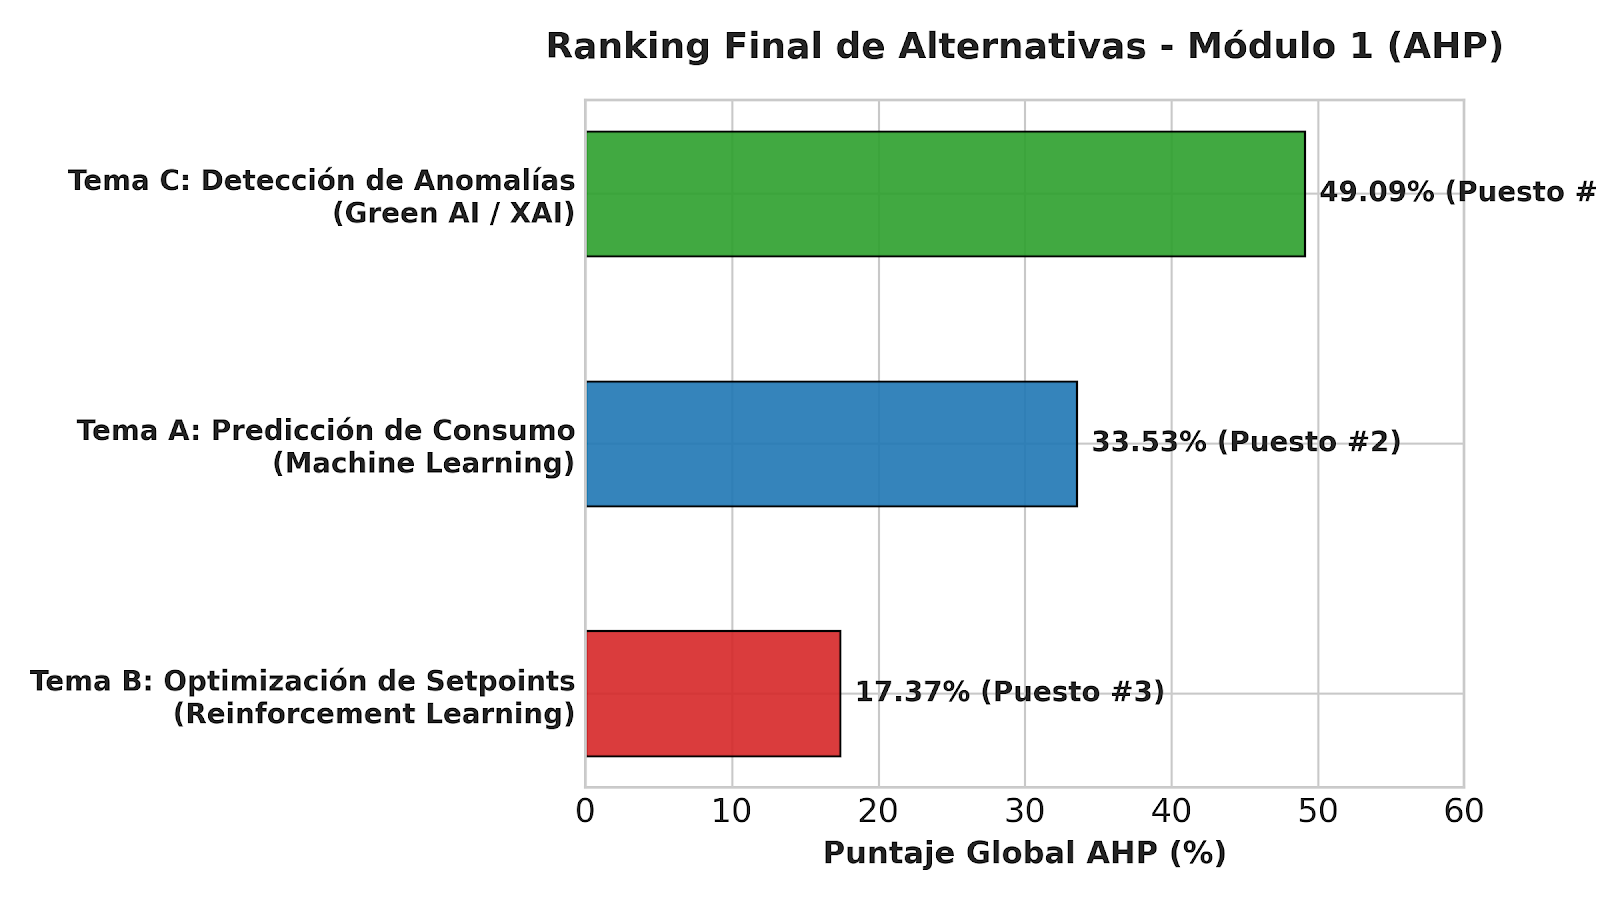
\includegraphics[width=0.78\textwidth]{ranking.png}
\caption{Ranking final de alternativas obtenido mediante AHP.}
\label{fig:ranking}
\end{figure}

\section{Discusión y Conclusiones}
El Tema C se impone de manera robusta frente a las demás alternativas \cite{giglio2024sand,ennen2025explainable}. A diferencia del Tema B, que presenta un elevado riesgo técnico por sim-to-real gap, y del Tema A, cuya formulación estándar ofrece bajo aporte de innovación, el Tema C equilibra alta factibilidad operativa con el paradigma Green AI \cite{schwartz2023green}, resultando el camino más sólido para el Trabajo Final de Carrera.

\bibliographystyle{splncs04}
\bibliography{mybibliography}

\end{document}
